\chapter{Einleitung}

Augmented Reality oder kurz AR ist eine computer-gestützte Erweiterung der Realitätswahrnehmung. Im Vergleich zur Virtual Reality wo der Anwender in eine komplett künstlich generierte Welt eintaucht, geht es bei AR primär darum zusätzliche Informationen anzuzeigen, welche sich bestmöglich in die Umgebung einpassen. AR kann alle menschlichen Sinne erweitern, jedoch beschränkt sich die heutige Technologie primär darauf Live-Bilder oder Videos mit Zusatzinformationen mittels Einblendung oder Überlagerung zu ergänzen.

\section{Anwendungsgebiete}

Augmented Reality kann in allen Bereichen des Alltags eingesetzt werden. Bei der Navigation im Auto oder im Gebäude können Routen und Hinweise direkt in die Umgebung integriert werden, so dass der Benutzer nie das Auge von der Strasse abwenden muss. Ärzten kann AR dabei helfen gezielter zu arbeiten indem Röntgen-aufnahmen während der Operation direkt auf den Patienten projiziert werden. Die Grundlagen hierfür sind meist die Gleichen wie in diesem Projekt. Objekterkennung, Positionsbestimmung und die Integration der Zusatzinformationen in die Umgebung.

\subsection{Medizin}

\begin{figure}[!ht]
\centering
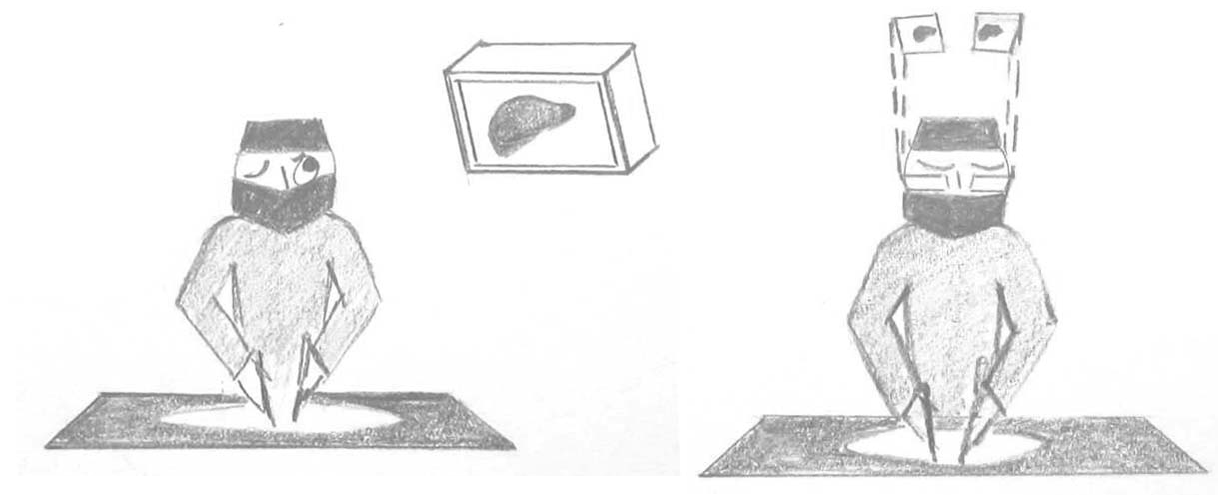
\includegraphics[scale=0.3]{images/vorteile_augmented_reality_medizin} 
\caption{Quelle: Suthau Tim, Berlin 2006, entnommen aus: Positionsgenaue Einblendung räumlicher Informationen in einem See Through Head Mounted Display für die Medizin am Beispiel der Leberchirurgie [Seite 13]}
\label{fig:ar-medicine}
\end{figure}

In der Medizin sind die Anwendungsmöglichkeiten von Augmented Reality vielfältig. Von der OP-Planung über die visuelle Navigation während der OP bis hin zur Telemedizin. Unterlagen wie Checklisten können zur Planung direkt Objektbezogen eingeblendet werden. So kann immer verfolgt werden wie die Vorbereitung des Patienten voranschreitet. Bei der Einrichtung des Operationssaales kann mittels AR direkt angezeigt werden, wo alles stehen muss um einen reibungslosen Ablauf der Operation zu garantieren. Während der Operation kann sich der Arzt voll und ganz auf den Patienten konzentrieren. Anstatt, dass er seinen Blick immer wieder abwenden muss um z.B. Röntgenaufnahmen zu betrachten, werden diese direkt in das Sichtfeld projiziert. Speziell bei minimalinvasiven Eingriffen können so auch direkt die Navigationswege dargestellt werden, was die Präzision des Eingriffes erhöht.
\paragraph{}
Im Bereich der Telemedizin können Spezialisten dem ausführenden Arzt Hilfestellungen während der Diagnose oder Operation einblenden. Mediziner können so in Weltweit in Echtzeit kooperieren.

\subsection{Marketing}

\begin{figure}[!ht]
\centering
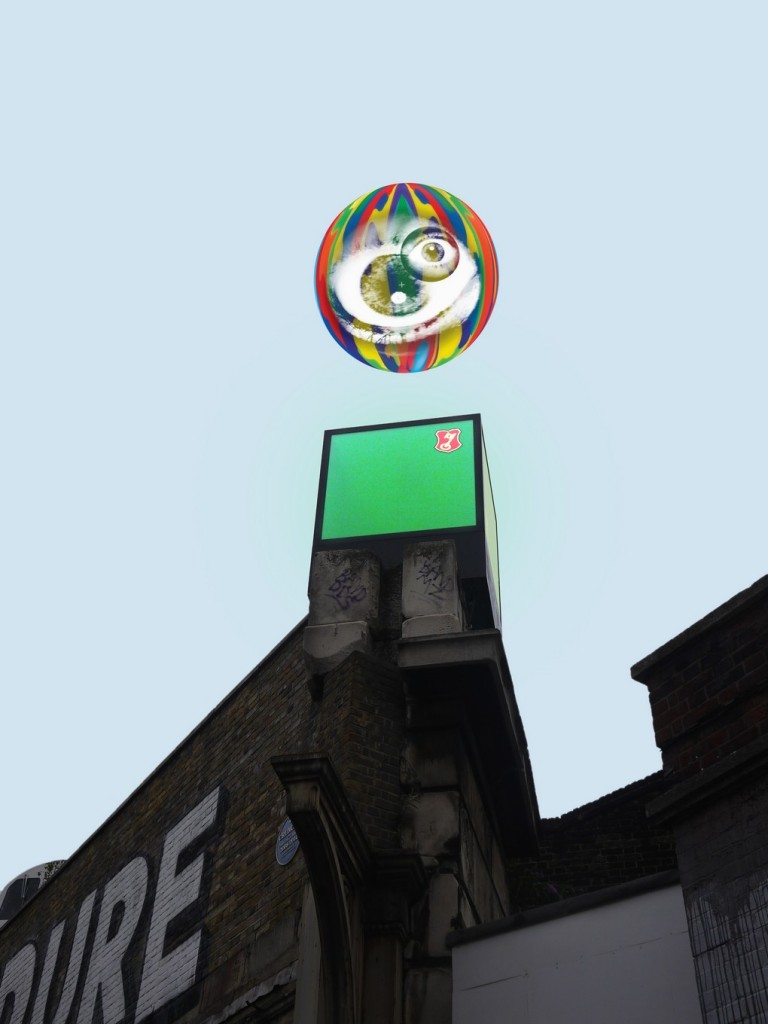
\includegraphics[scale=0.3]{images/ar-marketing} 
\caption{Becks Green Box Kampagne. Quelle: http://www.i-ref.de/2011/12/06/beck's-green-box-projekt-augmented-reality-in-berlin}
\label{fig:ar-marketing}
\end{figure}

Auch im Bereich des Marketing bietet Augented Reality unzählige neue Möglichkeiten. Tablets und Smartphones sind fester Bestandteil des Alltags geworden. Bietet man den Kunden die Möglichkeit Produkte und Brands interaktiv in ihrer Umgebung zu entdecken, so hinterlässt dies einen bleibenden Eindruck und erhöht die Bindung zur Marke. Ein Vorreiter war hier die Firma Becks im vergangenen Jahr. Um den Kunden das Produkt näher zu bringen hat Becks in Grossstädten weltweit grüne Boxen aufgestellt. Haben die Benutzer ihr Smartphone dann auf diese gerichtet, bot sich ihnen eine bunte 3D-Show. Direkt in ihrer gewohnten Umgebung im Herzen der Städte. Nach dieser Kampagne konnte Becks einen signifikaten Anstieg des Absatzes in der betroffenen Städten feststellen und gewann weltweit neue Fans.

\paragraph{}
Dies sind nur zwei mögliche Anwendungsgebiete. Bereits wird AR auch in der Automobilbranche in Form von Overhead Displays eingesetzt. Im Militärbereich wird AR für die Einsatzkoordination in Kriegsgebieten verwendet.

\section{Aktuelle Entwicklungen}

\begin{figure}[!ht]
\centering
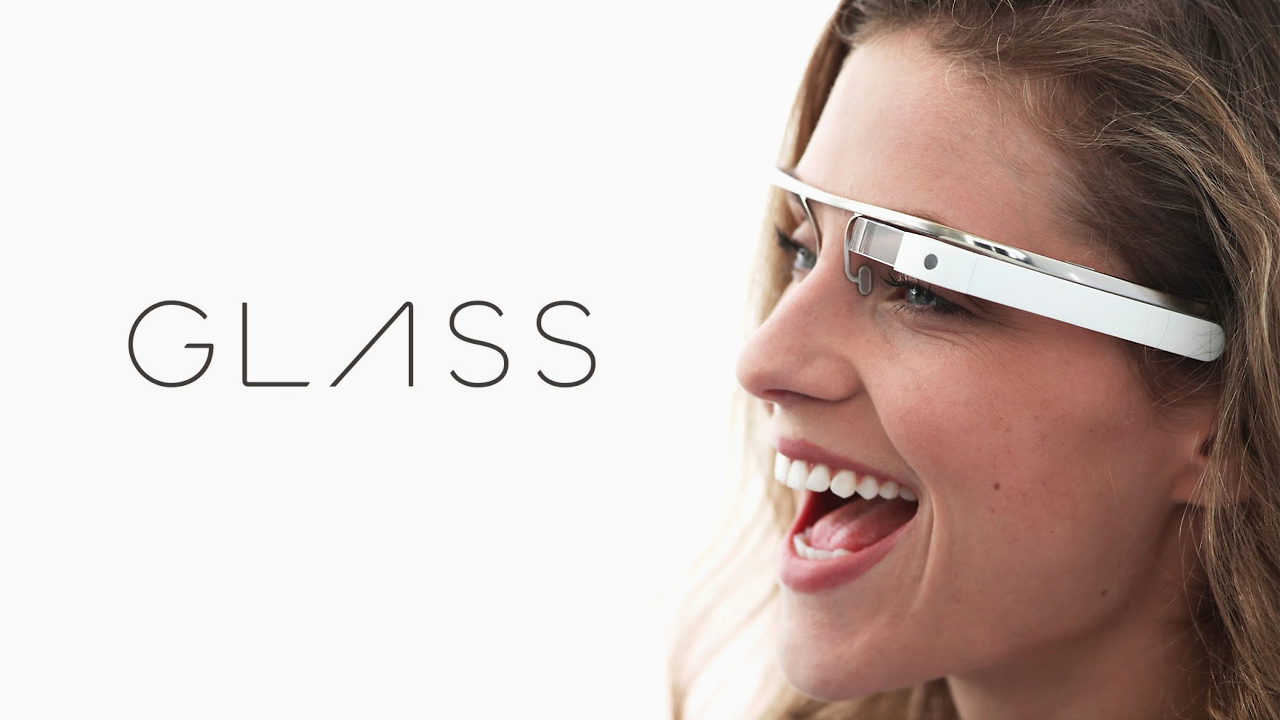
\includegraphics[width=\textwidth]{images/google-glass} 
\caption{Google Glass. Quelle: http://www.google.com/glass/start}
\label{fig:google-glass}
\end{figure}
\noindent
Bisher wurde das volle Potentiel von Augmented Reality nicht ausgeschöpft. Viele Anwendungen basieren immer noch auf sogenannten Markern, ähnlich wie QR-Codes, welche benötigt werden um zu bestimmen was und wo dargestellt werden muss. Die zweite Generation von AR-Applikationen ist jedoch auf den vormarsch. Diese können dank GPS und diverser anderer Sensoren in den Smartdevices auf Marker verzichten. Die Katalog-App von IKEA\footnote{\protect\url{http://mashable.com/2012/07/19/ikea-augmented-reality-catalog/}} und die TV Buying Guide App von Philips\footnote{\protect\url{http://www.youtube.com/watch?v=YBU0f0apgM0}} bauen beide auf diesen neuen Möglichkeiten auf. Augmented Reality Anwendungen haben im Jahr 2013 Weltweit schätzungweise einen Umsatz von \$300 Millionen generiert\footnote{\protect\url{Quelle: http://www.juniperresearch.com/viewpressrelease.php?pr=348}}.
\paragraph{}
Die zur Zeit fortschrittlichsten Anwendungen von AR sind im Bereich der tragbaren Devices zu finden, allen voran Google Glass\footnote{\protect\url{http://www.google.com/glass/start}}. Mit Glass integriert Google Smartphonefunktionalität in Brillen. Die Meta Glasses\footnote{\protect\url{https://www.spaceglasses.com/}} gehen noch einen Schritt weiter und integrieren einen dem Microsoft Kinect ähnliche Kamera, welche eine präzise Erkennung von Gesten erlauben soll. Dies soll eine Interaktion mit Augmented Reality Objekten erlauben. Das Produkt soll im Juli 2014 Marktreife erreichen. Apple und Microsoft haben diverse Patente eingereicht, welche darauf hindeuten, dass auch sie an entsprechendem Equipment arbeiten.